\documentclass[11pt]{article}
\usepackage[margin=1in]{geometry}
\usepackage{graphicx}
\usepackage{amsmath}
\usepackage{booktabs}

\title{A Finite Intercept Correction Calculation}
\author{Anonymous}
\date{}

\begin{document}
\maketitle

\begin{abstract}
This technical teaching note connects an additive intercept correction, its computed errors, and the observations used to obtain them. Five synthetic observations satisfy $y=2x+3$, while a fixed predictor returns $2x$. Their residual mean is $3$, so adding this constant reproduces every supplied target. At corrections $0$, $1.5$, and $3$, the computed mean squared errors are $9$, $2.25$, and $0$. A squared-error decomposition explains why removing a residual mean eliminates every error precisely when the residuals are constant. A table and two supplied figures make the calculation and its same-sample evaluation explicit.
\end{abstract}

\section{Introduction}

This note is intended for readers learning introductory regression and for a reproducible-workflow demonstration. Its instructional purpose is to connect three steps that can otherwise be read separately: computing a correction from residuals, explaining its effect on an error summary, and tracing which observations enter evaluation. The example is a worked application of established intercept-fitting algebra.

The learning objectives are to distinguish the supplied slope from the fitted additive constant, distinguish removing an average discrepancy from removing every discrepancy, and recognize the dependence created when correction and evaluation use the same targets. The small calculation allows each step to be checked by hand and compared with the generated artifacts.

For five inputs $x=(-2,-1,0,1,2)$, the supplied targets satisfy $y_i=2x_i+3$ and the fixed predictions are $2x_i$. Their difference is always $3$. Thus, exact agreement after correction follows directly from the specified targets and predictor. Throughout, reported errors describe this finite calculation on the supplied observations.

\section{Related Work}

Residual analysis uses discrepancies between responses and fitted values to examine a model's fit \cite{Anscombe1963ExaminationAnalysis}. This motivates displaying the residual vector before summarizing its errors. Treatments of regression through the origin discuss intercept omission and associated fitting and evaluation questions \cite{Eisenhauer2003RegressionThrough}. Here, the slope is supplied, so the arithmetic concerns only an additive constant.

Apparent-error analysis explains the dependence introduced by using observations both to fit a prediction rule and to assess its accuracy \cite{Efron1986HowBiased}. This supports the explicit observation-reuse path in the schematic. These references provide context for the teaching objectives; the numerical results follow from the supplied calculation.

\section{Method}
\subsection{Finite Setup and Mean-Residual Correction}

Retain the fixed predictor $\hat y_i^{(0)}=2x_i$ and define
\[
r_i=y_i-\hat y_i^{(0)},\qquad
\bar r=\frac{1}{5}\sum_{i=1}^{5}r_i,\qquad
\hat y_i(b)=2x_i+b.
\]
Here, $r_i=3$ for every observation and $\bar r=3$. The correction changes the intercept while preserving the slope.

The squared-error decomposition makes the role of the mean explicit:
\begin{equation}
\frac{1}{5}\sum_{i=1}^{5}(b-r_i)^2
=
\frac{1}{5}\sum_{i=1}^{5}(r_i-\bar r)^2
+(b-\bar r)^2.
\label{eq:decomposition}
\end{equation}
To obtain this identity, expand
$b-r_i=(b-\bar r)-(r_i-\bar r)$; the cross term vanishes because
$\sum_i(r_i-\bar r)=0$. Consequently, $b=\bar r$ minimizes squared error. The minimum equals the centered squared-residual term, which is zero exactly when every residual equals its mean. This distinguishes minimization from elimination: unequal residuals retain a positive centered term. In the supplied calculation, that term is zero because all residuals equal $3$.

\begin{figure}[htbp]
    \centering
    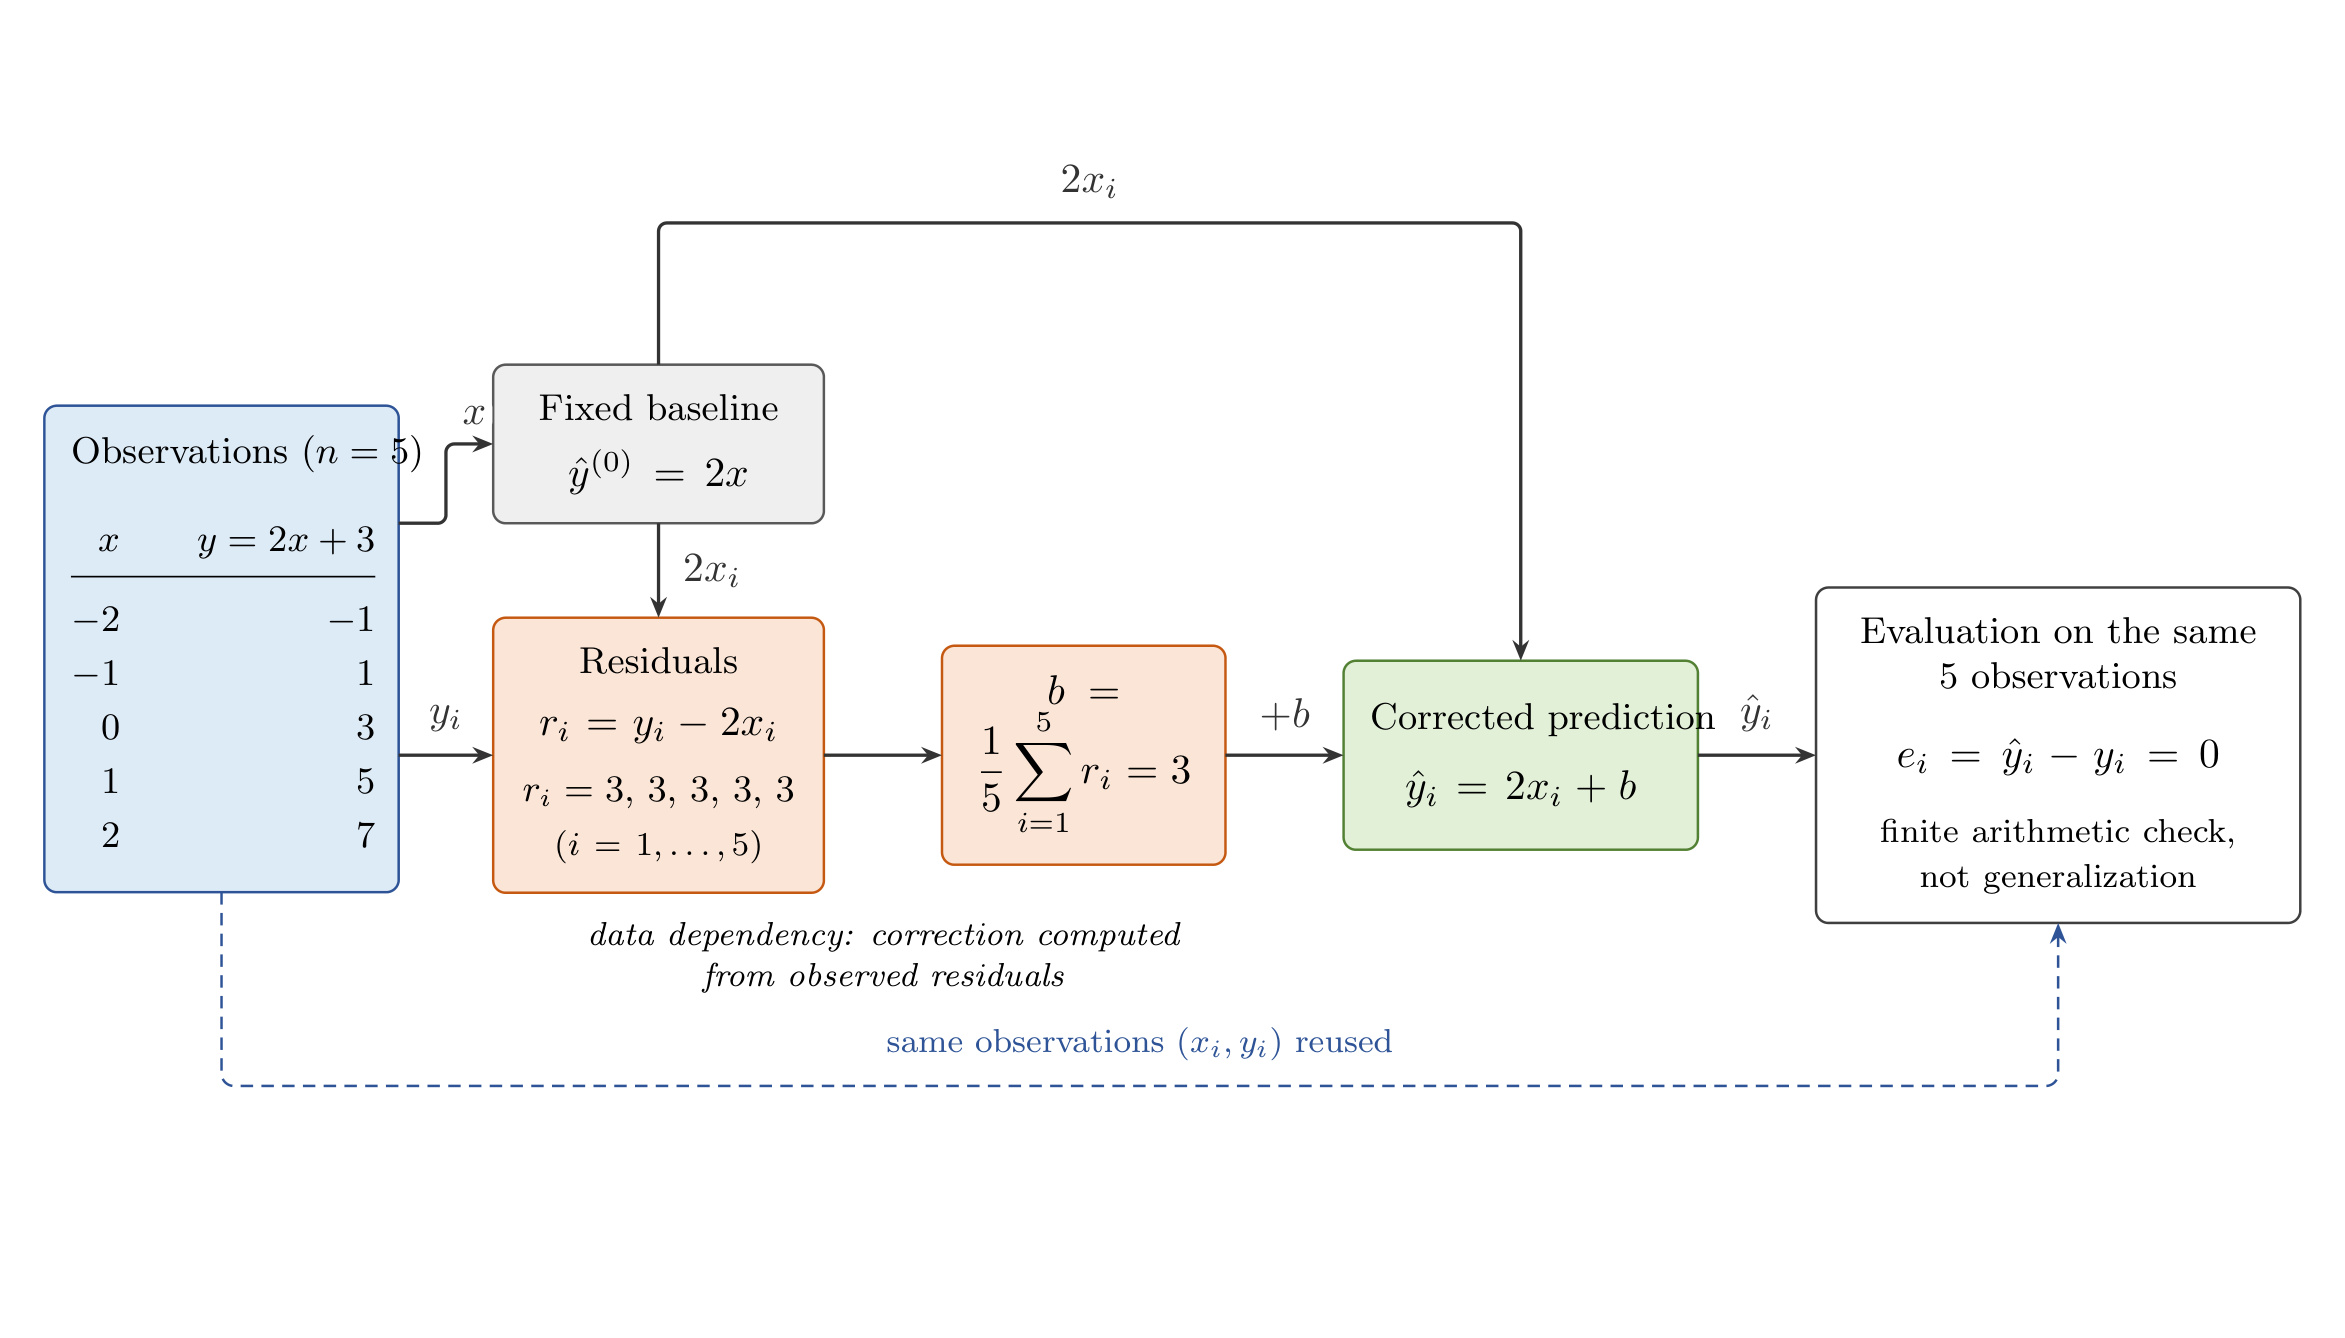
\includegraphics[width=\linewidth]{figures/fig_residual_workflow.jpg}
    \caption{Dependencies in the five-observation calculation. Targets and fixed predictions determine residuals and their mean correction. The dashed path shows reuse of the observations for evaluation. Baseline residuals use $r_i=y_i-2x_i$; corrected errors use $e_i=\hat y_i-y_i$.}
    \label{fig_residual_workflow}
\end{figure}

\subsection{Error Definitions and Reproducible Calculation}

Following the schematic, define corrected error as prediction minus target:
\[
e_i(b)=\hat y_i(b)-y_i=b-r_i=b-3.
\]
The baseline residual and corrected error therefore have explicitly different roles and signs. The reported summaries are
\begin{align}
\operatorname{MAE}(b)
&=\frac{1}{5}\sum_{i=1}^{5}|e_i(b)|=|b-3|,\\
\operatorname{MSE}(b)
&=\frac{1}{5}\sum_{i=1}^{5}e_i(b)^2=(b-3)^2.
\end{align}
Reversing the error sign leaves both summaries unchanged. The numerical calculation uses base R \cite{Ihaka1996RLanguage}; the statistical plot uses R/ggplot2 \cite{Wickham2009LayeredGrammar}.

\section{Experiments}
\subsection{Observations and Evaluation Protocol}

The supplied calculation contains the following rows:
\[
\begin{array}{c|rrrrr}
x & -2 & -1 & 0 & 1 & 2\\
y & -1 & 1 & 3 & 5 & 7\\
2x & -4 & -2 & 0 & 2 & 4\\
2x+3 & -1 & 1 & 3 & 5 & 7
\end{array}
\]
One deterministic computation evaluates three recorded settings: the baseline $b=0$, an intermediate correction $b=1.5$, and the residual-mean correction $b=3$. The same five targets determine $\bar r$ and enter every error summary. These are computed values from fully specified synthetic inputs.

\subsection{Recorded Errors and Their Interpretation}

Table~\ref{tab_recorded_errors} gives the computed errors. At $b=0$, every prediction-minus-target error equals $-3$. At $b=1.5$, every error equals $-1.5$, giving MAE $1.5$ and MSE $2.25$. At $b=3$, each corrected prediction equals its target.

\begin{table}[htbp]
    \centering
    \caption{Computed errors on the same five observations used to determine the residual-mean correction.}
    \label{tab_recorded_errors}
    \begin{tabular}{@{}rrr@{}}
        \toprule
        Added $b$ & Mean absolute error & Mean squared error\\
        \midrule
        0   & 3   & 9\\
        1.5 & 1.5 & 2.25\\
        3   & 0   & 0\\
        \bottomrule
    \end{tabular}
\end{table}

\begin{figure}[htbp]
    \centering
    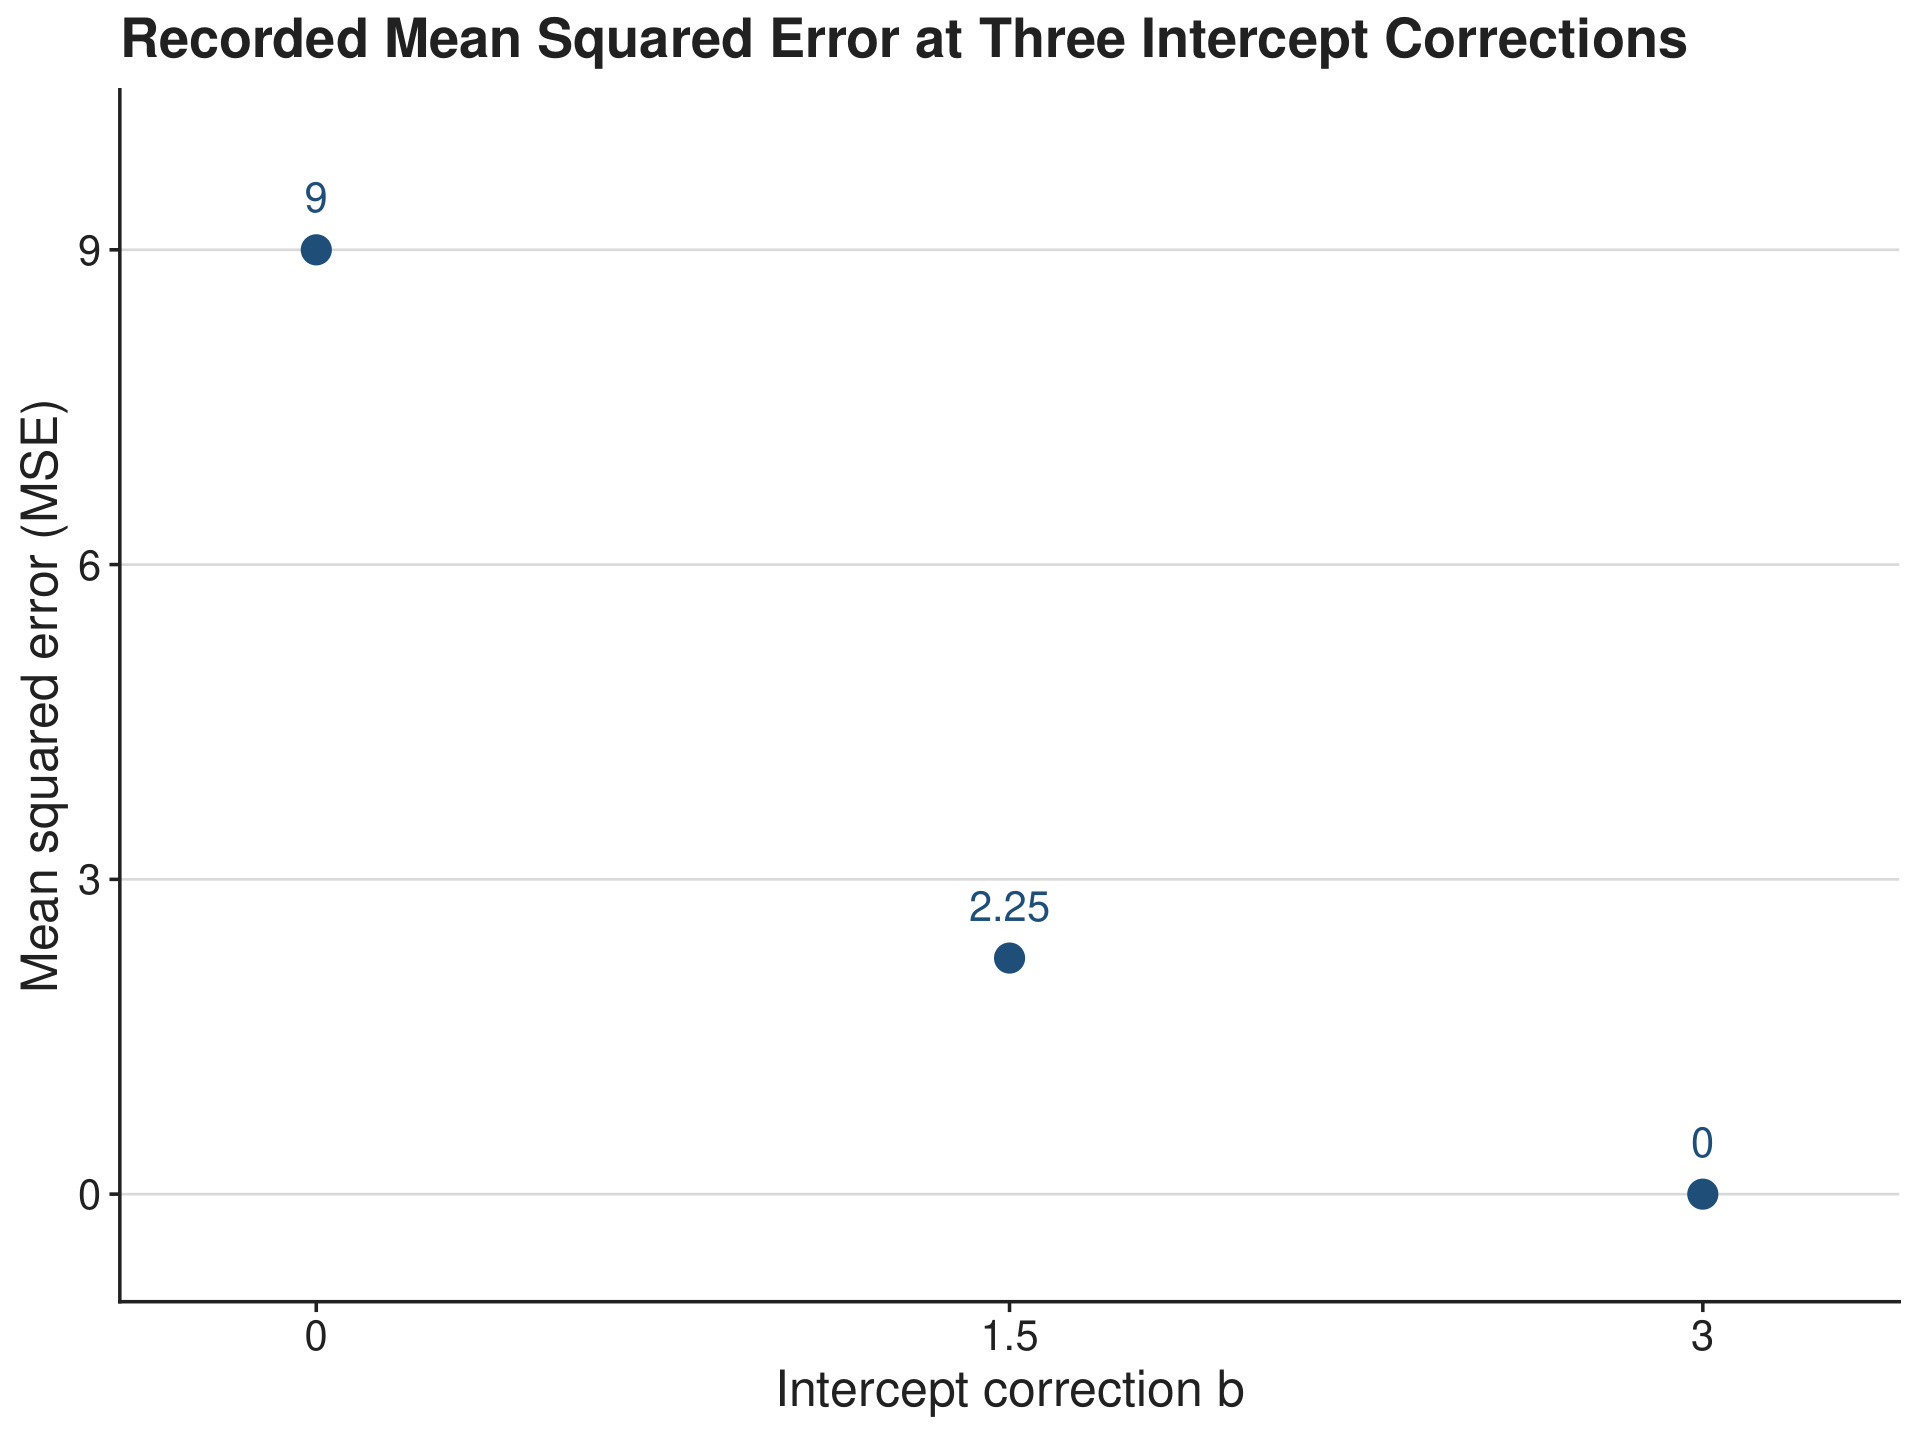
\includegraphics[width=0.9\linewidth]{figures/fig_intercept_error.jpg}
    \caption{The three recorded MSE values at $b=0$, $1.5$, and $3$. Each labeled point evaluates the fixed-slope predictor on the supplied five observations.}
    \label{fig_intercept_error}
\end{figure}

Figure~\ref{fig_intercept_error} displays exactly these three recorded settings. Equation~\ref{eq:decomposition} explains their arithmetic, while Figure~\ref{fig_residual_workflow} explains their data dependence. Their agreement verifies the finite computation. The pedagogical reading is therefore twofold: the residual mean selects the squared-error-minimizing constant, and the constant residual vector explains the resulting same-sample zero error.

\section{Conclusion}

The example links a residual vector, an additive correction, computed error summaries, and an explicit evaluation dependency. Adding $b=3$ reproduces the five targets because every baseline residual equals $3$. The decomposition identifies the condition for this exact agreement and distinguishes it from merely minimizing squared error. Together, the equations, table, and supplied figures form a checkable introductory workflow.


\bibliographystyle{plain}
\bibliography{references}

% PAPER_ORCHESTRA_PROVENANCE_BEGIN
\clearpage
\section*{Figure source provenance}
The files below are the exact sources that produced the embedded figure previews. Paths are relative to this manuscript's source directory. The accompanying \texttt{figure\char95{}provenance.json} records all artifact checksums.\par
\medskip\noindent\textbf{Figure~\ref{fig_intercept_error} (\texttt{fig\char95{}intercept\char95{}error.jpg}).}\par
\noindent R/ggplot2 source: \texttt{figure\char95{}code/\allowbreak{}fig\char95{}intercept\char95{}error/\allowbreak{}source.R}.\par
\noindent Source SHA256: \texttt{68963e7e\allowbreak{}0f21eaa5\allowbreak{}7dfe9d41\allowbreak{}50f6248f\allowbreak{}d142e763\allowbreak{}e30835f3\allowbreak{}e6e8af10\allowbreak{}adc25ae2}.\par
\noindent Rendering metadata: \texttt{figure\char95{}code/\allowbreak{}fig\char95{}intercept\char95{}error/\allowbreak{}render.json}.\par
\noindent Exact export wrapper: \texttt{figure\char95{}code/\allowbreak{}fig\char95{}intercept\char95{}error/\allowbreak{}worker.R}.\par
\noindent Wrapper SHA256: \texttt{6cb2b073\allowbreak{}27277f63\allowbreak{}fafbb553\allowbreak{}cd4f1f12\allowbreak{}c0f85bec\allowbreak{}37a49f3f\allowbreak{}a765da16\allowbreak{}a26b58ba}.\par
\noindent Rendering metadata: \texttt{figure\char95{}code/\allowbreak{}fig\char95{}intercept\char95{}error/\allowbreak{}sessionInfo.txt}.\par
\medskip\noindent\textbf{Figure~\ref{fig_residual_workflow} (\texttt{fig\char95{}residual\char95{}workflow.jpg}).}\par
\noindent LaTeX/TikZ source: \texttt{figure\char95{}code/\allowbreak{}fig\char95{}residual\char95{}workflow/\allowbreak{}source.tex}.\par
\noindent Source SHA256: \texttt{66606680\allowbreak{}7053c57a\allowbreak{}dee8b194\allowbreak{}7e99adeb\allowbreak{}6a9369c3\allowbreak{}c53399fd\allowbreak{}76a38033\allowbreak{}1907dee2}.\par
\noindent Rendering metadata: \texttt{figure\char95{}code/\allowbreak{}fig\char95{}residual\char95{}workflow/\allowbreak{}render.json}.\par
% PAPER_ORCHESTRA_PROVENANCE_END
\end{document}